\chapter{统计热力学：配分函数}\label{ch:b3:partition-functions}

维也纳的玻尔兹曼墓碑上只刻着一行字：$S = k\log W$，
体系的熵，计算的是其分子分享能量的方式数。
热力学在本科一年级和二年级分册中如此建立，从不需要分子：
它只把可测的热量、熵和平衡常数相互联系起来。
统计热力学则从分子本身出发计算这些量。
其核心对象是对单个分子能级求和得到的一个式子，
即配分函数；能级由光谱学给出，
由光谱算得的氮气标准摩尔熵与表列值一致，
误差在百分之一焦耳每开尔文每摩尔以内。本章
建立配分函数，将其拆分为平动、转动、
振动和电子部分，并由此导出内能、熵
和吉布斯自由能；\cref{ch:b3:statistical-thermo-applied} 将其用于热
容与平衡常数。

\begin{recall}
本科二年级分册定义了标准摩尔熵、吉布斯自由能和
化学势，并列出了由热容求得的熵值，
其测量延伸至低温。\Cref{ch:b3:quantum-model-systems} 给出了
势箱中粒子、谐振子和
刚性转子的能级，$E_J = hcBJ(J+1)$，简并度为 $2J + 1$；
\cref{ch:b3:rovibrational-spectroscopy} 测量了双原子分子的 $B$ 与 $\tilde\nu$，
并发现在 \ce{N2} 这类同核分子中，
核自旋使相邻的转动能级不等价。
\end{recall}

\section{微观态与玻尔兹曼分布}

设 $N$ 个相同且相互独立的分子，可占据能量为
$\varepsilon_0 = 0 < \varepsilon_1 < \varepsilon_2 < \dots$ 的能级，总能量为 $E$。说明每个能级上有多少分子，
即 $\{n_0, n_1, \dots\}$，描述的是一种分布；
说明哪个分子处于哪个能级，则描述得多得多。

\begin{definition}[微观态，统计权重]\label{def:b3:partition-functions:microstate}
分子体系的一个\emph{微观态}\index{微观态}，
是对每个分子状态的完整指定。其\emph{统计权重}\index{统计权重}
$W$ 为分布 $\{n_i\}$ 的
统计权重，即 $N$ 个分子在非简并能级上实现该分布的微观态数目：
\[
  W = \frac{N!}{n_0!\,n_1!\,n_2!\cdots}.
\]
\end{definition}

\begin{example}[三个振子共享三个量子]\label{ex:b3:partition-functions:three-quanta}
三个振子共享三个能量量子。分布“一个振子占有全部三个量子”
可以用 $3!/(1!\,2!) = 3$ 种方式实现，“一个振子占有两个，另一个占有一个”
有 $3! = 6$ 种方式，“每个振子各占一个”只有一种方式：
共计十个微观态。在仍使能量分布于若干能级上的分布中，
最均匀的那个最可能出现。对于 $10^{23}$ 个分子，
权重变得极为尖锐，以至于这一分布以及与之只相差可忽略量的分布，
几乎占据了全部微观态。
\end{example}

\begin{remark}
统计热力学的基本假设是：一个孤立体系在给定能量下的全部
微观态等概率。于是，体系几乎总是处于权重最大的分布之中，
求出这一分布，
正是本节的任务。
\end{remark}

对于大数，斯特林近似 $\ln x! \approx x\ln x - x$ 给出
\[
  \ln W = N\ln N - \sum_i n_i\ln n_i .
\]

\begin{definition}[玻尔兹曼分布，布居数]\label{def:b3:partition-functions:boltzmann}
能级的\emph{布居数}\index{布居数} $n_i/N$ 是占据该能级的
分子所占的比例。\emph{玻尔兹曼分布}\index{玻尔兹曼分布}
是独立分子在热平衡下具有最大权重的分布，
该热平衡温度为 $T$，由下面的定理给出。
\end{definition}

\begin{theorem}[玻尔兹曼分布]\label{thm:b3:partition-functions:boltzmann}
对于温度为 $T$ 的热平衡下的独立分子，
能量为 $\varepsilon_i$、简并度为 $g_i$ 的能级，其布居数为
\[
  \frac{n_i}{N} = \frac{g_i\eu^{-\varepsilon_i/kT}}{q},
  \qquad q = \sum_i g_i\eu^{-\varepsilon_i/kT},
\]
其中 $k$ 为玻尔兹曼常数。两能级的布居数之比为
$\frac{n_j}{n_i} = \frac{g_j}{g_i}\eu^{-(\varepsilon_j - \varepsilon_i)/kT}$.
\end{theorem}

\begin{proof}[部分证明]
先考虑非简并能级。对 $\ln W$ 求极大，
约束为 $\sum_in_i = N$ 和 $\sum_in_i\varepsilon_i = E$，拉格朗日乘子为 $\alpha$ 和 $\beta$：
对每个 $i$，
\[
  \frac{\partial}{\partial n_i}\Bigl(\ln W + \alpha\sum_jn_j - \beta\sum_jn_j\varepsilon_j\Bigr)
  = -\ln n_i - 1 + \alpha - \beta\varepsilon_i = 0,
\]
于是 $n_i = \eu^{\alpha - 1}\eu^{-\beta\varepsilon_i}$，由第一个约束得 $\eu^{\alpha - 1}
= N/\sum_j\eu^{-\beta\varepsilon_j}$。简并度为 $g_i$ 的能级包含 $g_i$ 个能量相同的不同状态，
每个状态的布居数如上式所示，其布居数乘以
$g_i$。乘子 $\beta$ 由一个已知情形确定：
对理想气体的平动（见下文\cref{prop:b3:partition-functions:q-trans}
）该分布给出能量 $\frac32N/\beta$，而理想气体的能量为
$\frac32NkT$，故 $\beta = 1/kT$。此 $\beta$ 对一切运动形式都是同一个量，
各种运动形式都如此；它即热力学温度，这一点在此予以承认：
两个处于热接触的体系具有相同的 $\beta$，这
正是温度的定义性质。
\end{proof}

\begin{definition}[分子配分函数]\label{def:b3:partition-functions:partition-function}
分子的\emph{分子配分函数}\index{分子配分函数}
在温度为 $T$ 时，为如下求和：
\[
  q = \sum_{\text{能级}}g_i\eu^{-\varepsilon_i/kT} = \sum_{\text{状态}}\eu^{-\varepsilon_s/kT},
\]
能量从最低能级算起，因此 $q \ge 1$。
\end{definition}

配分函数统计在热力学上可以到达的状态数：
在极低温度下，只有最低能级有贡献，$q \to g_0$；在极高温度下，
每个状态的贡献都约为 1，$q$ 无限增大。
由此得出一条经验规则：比最低能级高出远大于 $kT$ 的能级几乎无人占据，
距最低能级在 $kT$ 之内的能级则有粒子占据。在 \qty{298.15}{K} 下，$kT$
相当于 \qty{207.2}{cm^{-1}}，或 $RT = \qty{2.479}{kJ/mol}$。

\begin{method}[由光谱常数求能级占据数]\label{met:b3:partition-functions:populations}
\begin{enumerate}
  \item 列出各能级的能量（由常数求得，例如
        $hcBJ(J+1)$）及简并度（$2J + 1$）。
  \item 将各能量以 $kT$ 为单位表示；在 \qty{298.15}{K} 下，把
        波数除以 \qty{207.2}{cm^{-1}}。
  \item 计算各项 $g_i\eu^{-\varepsilon_i/kT}$，求和得 $q$，再相除。
        各项可以忽略时停止求和。
  \item 检验：各占据数之和为 1；任意两个占据数之比为
        $\frac{g_j}{g_i}\eu^{-(\varepsilon_j-\varepsilon_i)/kT}$。
\end{enumerate}
\end{method}

\begin{example}[氯化氢的转动能级]\label{ex:b3:partition-functions:hcl}
% ledger: diat:HCl.Be, diat:HCl.ae
对于 \ce{H^{35}Cl}，$B_0 = B_e - \alpha_e/2 = \qty{10.44}{cm^{-1}}$。在 \qty{300}{K} 下，能级 $J$
位于 $10.44\,J(J+1)$~\unit{cm^{-1}}，即 $0.0501\,J(J+1)$，单位为 $kT$。各项
$(2J+1)\eu^{-0.0501J(J+1)}$ 依次为 1、2.71、3.70、3.84、3.31、2.45、\dots；其和为
$q = 20.3$，$J = 0$ 至 4 的占据数分别为 0.049、0.134、0.182、0.189 和
0.163。占据数最大的是 $J = 3$ 而非 $J = 0$，原因在于简并度
$2J + 1$ 增长而玻尔兹曼因子下降。这正是
\cref{ch:b3:rovibrational-spectroscopy}中振转光谱带的包络。
\end{example}

\begin{omfigure}
\begin{tikzpicture}[font=\small]
  % levels J = 0-3, g = 2J+1, energies 0, 1, 3, 6 (units of 2hcB); bars = 3.5 cm x population
  % of the four levels alone at kT = 2hcB (0.422, 0.466, 0.105, 0.007) and kT = 10hcB (0.120, 0.296, 0.330, 0.254)
  \foreach \J/\e/\g/\lo/\hi in {0/0/1/1.48/0.42, 1/1/3/1.63/1.04, 2/3/5/0.37/1.16, 3/6/7/0.03/0.89}{
    \draw[thick] (0,0.55*\e) -- (2.2,0.55*\e);
    \node[anchor=east] at (0,0.55*\e) {$J = \J$};
    \node[anchor=west, font=\scriptsize] at (2.25,0.55*\e) {$g = \g$};
    \fill[omDef!70] (3.4,0.55*\e-0.11) rectangle ++(\lo,0.22);
    \fill[omThm!70] (6.4,0.55*\e-0.11) rectangle ++(\hi,0.22);
  }
  \node[anchor=south, omDef] at (4.2,3.6) {低 $T$};
  \node[anchor=south, omThm] at (7.2,3.6) {高 $T$};
  \draw[->] (-1.4,0) -- (-1.4,3.7) node[anchor=south] {$\varepsilon$};
\end{tikzpicture}

{\small 玻尔兹曼阶梯：转动能级 $J = 0$ 至 3（能量分别为 $0$、$2$、$6$、
$12$ 倍 $hcB$，简并度 $2J + 1$），及其占据数（以条形长度表示），
分别取 $kT = 2hcB$ 和 $kT = 10hcB$（仅计这四个能级）。升温使
粒子从最低能级移向较高能级；两种温度下条形之和相同，
均等于分子总数。}
\end{omfigure}

\section{分子配分函数}

\begin{proposition}[因子分解]\label{prop:b3:partition-functions:factorisation}
若分子的能量是若干独立贡献之和，
$\varepsilon = \varepsilon^{\mathrm T} + \varepsilon^{\mathrm R} + \varepsilon^{\mathrm V} + \varepsilon^{\mathrm E}$，每个状态
都是平动、转动、振动与电子状态的任意组合，
则
\[
  q = q^{\mathrm T}q^{\mathrm R}q^{\mathrm V}q^{\mathrm E}.
\]
\end{proposition}

\begin{proof}
对一个和的指数在所有组合上求和，等于各部分单独求和的乘积，
即 $\sum_{a,b}\eu^{-(\varepsilon_a+\varepsilon_b)/kT} = \bigl(\sum_a\eu^{-\varepsilon_a/kT}\bigr)
\bigl(\sum_b\eu^{-\varepsilon_b/kT}\bigr)$，对四个因子同理。
\end{proof}

这种分离只是近似：转动与振动相互作用（
常数 $\alpha_e$），电子状态则决定转动与振动的
常数。对于处于基电子态、常温下的分子，
熵的误差仅约为每开尔文百分之几焦耳。因此，
各类运动的占据数应分别计算：
振动能级 $v$ 上的分子占比
与其转动状态无关。

\section{四项贡献}

\subsection*{平动}

\begin{definition}[热波长]\label{def:b3:partition-functions:thermal-wavelength}
质量为 $m$ 的分子在温度 $T$ 下的\emph{热波长}\index{热波长}为
$\Lambda = \dfrac{h}{\sqrt{2\pi mkT}}$。
\end{definition}

\begin{proposition}[平动配分函数]\label{prop:b3:partition-functions:q-trans}
对于质量为 $m$、可在体积 $V$ 内自由运动的分子，
\[
  q^{\mathrm T} = \frac{V}{\Lambda^3}.
\]
\end{proposition}

\begin{proof}
对于一维情形，长为 $L$ 的箱子中能级为 $\varepsilon_n = h^2n^2/8mL^2$
（$n = 1, 2, \dots$；零点能的整体偏移不影响任何可测结果）。这些能级非常
靠近，因此求和可以写成积分：
\[
  q_x = \sum_{n\ge1}\eu^{-h^2n^2/8mL^2kT} \approx \int_0^\infty\eu^{-h^2n^2/8mL^2kT}\dd n
      = \frac12\sqrt{\frac{\pi\,8mL^2kT}{h^2}} = \frac{L\sqrt{2\pi mkT}}{h} = \frac{L}{\Lambda}.
\]
三个方向相互独立：$q^{\mathrm T} = q_xq_yq_z = L^3/\Lambda^3$。每个
方向的平均能量为 $-\partial\ln q_x/\partial\beta$，其中 $q_x \propto \beta^{-1/2}$，即
$1/2\beta$；三个方向共给出每个分子 $\frac32kT$，正是
\cref{thm:b3:partition-functions:boltzmann}证明中所用的结果。
\end{proof}

\begin{example}[烧瓶中的氩]\label{ex:b3:partition-functions:argon}
% ledger: aw:Ar, const:h, const:kB
对于氩（$M = \qty{39.95}{g/mol}$），在 \qty{298.15}{K} 下，$\Lambda = \qty{16.0}{pm}$，
约为一个原子直径的十分之一。在 \qty{1}{dm^3} 中，$q^{\mathrm T} = 10^{-3}/(1.600\times10^{-11})^3 = \num{2.44e29}$
可被热激发的平动状态远多于
烧瓶在 \qty{1}{bar} 下所含的 $2.4\times10^{22}$ 个原子：每个状态几乎总是
空的，这正是下文把分子当作可数对象来处理的前提。
\end{example}

\subsection*{转动}

\begin{definition}[特征温度]\label{def:b3:partition-functions:characteristic-temperature}
对转动常数为 $B$ 的线性分子，其\emph{转动特征温度}\index{转动特征温度}
为 $\theta_{\mathrm R} =
hcB/k$；对波数为 $\tilde\nu$ 的振动，其\emph{振动特征温度}\index{振动特征温度}
为 $\theta_{\mathrm V} =
hc\tilde\nu/k$。
\end{definition}

\begin{definition}[对称数]\label{def:b3:partition-functions:symmetry-number}
分子的\emph{对称数}\index{对称数} $\sigma$ 是
刚性分子经真转动可到达、且与初始构型不可区分的
不同取向的数目（即其点群中转动子群的阶）：
对 \ce{HCl} 与 \ce{CO} 为 1；对 \ce{N2}、
\ce{CO2} 与 \ce{H2O} 为 2；对 \ce{NH3} 为 3；对 \ce{CH4} 与 \ce{C6H6} 为 12。
\end{definition}

\begin{proposition}[转动配分函数]\label{prop:b3:partition-functions:q-rot}
对线性分子，$q^{\mathrm R} = \sum_J(2J+1)\eu^{-\theta_{\mathrm R}J(J+1)/T}$。当 $T \gg
\theta_{\mathrm R}$ 时，
\[
  q^{\mathrm R} \approx \frac{T}{\sigma\theta_{\mathrm R}} = \frac{kT}{\sigma hcB},
\]
此时相对误差约为 $\theta_{\mathrm R}/3T$（取 $\sigma = 1$，精确求和接近
$T/\theta_{\mathrm R} + \frac13$）。
\end{proposition}

\begin{proof}[部分证明]
当 $T \gg \theta_{\mathrm R}$ 时，参与贡献的能级很多，求和化为积分。
令 $x = J(J+1)$，则 $\dd x = (2J+1)\dd J$：
\[
  \int_0^\infty(2J+1)\eu^{-\theta_{\mathrm R}J(J+1)/T}\dd J = \int_0^\infty\eu^{-\theta_{\mathrm R}x/T}\dd x
  = \frac{T}{\theta_{\mathrm R}}.
\]
修正项 $\frac13$ 来自欧拉–麦克劳林公式的下一项
（见\cref{exo:b3:partition-functions:11}）。因子 $1/\sigma$ 在此予以承认，
并在\cref{ch:b3:statistical-thermo-applied}中加以论证：在同核分子中，
波函数在两个相同原子核交换下的对称性
使每个核自旋态只允许一种 $J$ 的奇偶性
（见\cref{ch:b3:rovibrational-spectroscopy}），因此平均而言一半的转动
能级缺失。以这种方式用 $\sigma$ 计数转动态时，
$q$ 中不计核自旋态；热力学数据表遵循
同样的约定，核自旋因子在每一个化学
反应中都相互抵消。
\end{proof}

对 \ce{N2}，$B_0 = \qty{1.990}{cm^{-1}}$ 和 $\theta_{\mathrm R} = \qty{2.86}{K}$：在 \qty{298.15}{K} 下，
$q^{\mathrm R} = 298.15/(2\times2.863) = 52.1$。对 \ce{HCl}，$\theta_{\mathrm R} = \qty{15.0}{K}$，
$q^{\mathrm R} = 19.8$（精确求和为 20.2）。仅 \ce{H2}（$\theta_{\mathrm R} = \qty{85}{K}$）及其同位素异构体
在室温下需用精确求和。非线性分子的
转动常数为 $A$、$B$、$C$，则 $q^{\mathrm R} = \frac{1}{\sigma}\bigl(\frac{kT}{hc}\bigr)^{3/2}\sqrt{\frac{\pi}{ABC}}$，此式不加证明地承认。

\subsection*{振动}

\begin{proposition}[振动配分函数]\label{prop:b3:partition-functions:q-vib}
对波数为 $\tilde\nu$ 的简谐振动，能量自
零点能级算起，
\[
  q^{\mathrm V} = \sum_{v\ge0}\eu^{-v\theta_{\mathrm V}/T} = \frac{1}{1 - \eu^{-\theta_{\mathrm V}/T}} .
\]
当 $T \ll \theta_{\mathrm V}$ 时趋于 1；趋于 $T/\theta_{\mathrm V}$ 的情形则出现在 $T \gg \theta_{\mathrm V}$ 时。一个分子
含若干简正模式时，其配分函数为每个模式对应因子的乘积。
\end{proposition}

\begin{proof}
各能级高出零点能级 $v\,hc\tilde\nu$：求和是一个
公比为 $\eu^{-\theta_{\mathrm V}/T} < 1$ 的等比级数。当 $T \gg \theta_{\mathrm V}$ 时，$1 - \eu^{-\theta_{\mathrm V}/T} \approx \theta_{\mathrm V}/T$。
简正模式相互独立（见\cref{prop:b3:partition-functions:factorisation}）。
\end{proof}

对双原子分子的振动量子，本书取
实测基频 $G(1) - G(0) = \omega_e - 2\omega_ex_e$
（见\cref{ch:b3:rovibrational-spectroscopy}）。在室温下只需考虑最低的
几个能级，起作用的是它们的间距。刚性大、质量轻的分子
处于“冻结”状态：\ce{N2} 的 $\theta_{\mathrm V} = \qty{3352}{K}$，在 \qty{298.15}{K} 下 $q^{\mathrm V} = 1.000013$，
每一百万个分子中只有 13 个处于 $v = 1$。质量大、较软的分子则不然：\ce{I2}
的 $\theta_{\mathrm V} = \qty{307}{K}$，$q^{\mathrm V} = 1.556$，其中三分之一以上的分子
在振动。

\begin{omfigure}
\begin{tikzpicture}
\begin{axis}[name=rotA, width=0.36\linewidth, height=5.0cm, xmin=-0.5, xmax=14.5,
  ymin=0, ymax=0.34, axis lines=left, ycomb, xlabel={$J$}, ylabel={布居数},
  tick label style={font=\scriptsize}, label style={font=\small},
  title={\small \ce{HCl}, 转动}, scaled y ticks=false,
  yticklabel style={/pgf/number format/fixed}]
\addplot[omDef, line width=1.6pt, xshift=-1.6pt] table[x=J, y=T100] {figdata/out/bachelor-3-boltzmann-populations-hcl.dat};
\addplot[black!60, line width=1.6pt] table[x=J, y=T300] {figdata/out/bachelor-3-boltzmann-populations-hcl.dat};
\addplot[omThm, line width=1.6pt, xshift=1.6pt] table[x=J, y=T1000] {figdata/out/bachelor-3-boltzmann-populations-hcl.dat};
\end{axis}
\begin{axis}[name=rotB, at={(rotA.east)}, anchor=west, xshift=0.9cm, width=0.36\linewidth,
  height=5.0cm, xmin=-1, xmax=41, ymin=0, ymax=0.17, axis lines=left, ycomb,
  xlabel={$J$}, tick label style={font=\scriptsize}, label style={font=\small},
  title={\small \ce{CO}, 转动}, scaled y ticks=false,
  yticklabel style={/pgf/number format/fixed}]
\addplot[omDef, sharp plot, thin, mark=*, mark size=0.9pt] table[x=J, y=T100] {figdata/out/bachelor-3-boltzmann-populations-co.dat};
\addplot[black!60, sharp plot, thin, mark=*, mark size=0.9pt] table[x=J, y=T300] {figdata/out/bachelor-3-boltzmann-populations-co.dat};
\addplot[omThm, sharp plot, thin, mark=*, mark size=0.9pt] table[x=J, y=T1000] {figdata/out/bachelor-3-boltzmann-populations-co.dat};
\end{axis}
\begin{axis}[at={(rotB.east)}, anchor=west, xshift=0.9cm, width=0.32\linewidth,
  height=5.0cm, xmin=-0.5, xmax=10.5, ymin=0, ymax=0.7, axis lines=left, ycomb,
  xlabel={$v$}, tick label style={font=\scriptsize}, label style={font=\small},
  title={\small \ce{I2}, 振动}, scaled y ticks=false,
  yticklabel style={/pgf/number format/fixed}]
\addplot[black!60, line width=1.6pt, xshift=-1.2pt] table[x=v, y=T300] {figdata/out/bachelor-3-boltzmann-populations-i2.dat};
\addplot[omThm, line width=1.6pt, xshift=1.2pt] table[x=v, y=T1000] {figdata/out/bachelor-3-boltzmann-populations-i2.dat};
\end{axis}
\end{tikzpicture}

{\small 由光谱常数计算得到的玻尔兹曼布居数：
\ce{H^{35}Cl} 的转动能级（$\theta_{\mathrm R} = \qty{15.0}{K}$）和 \ce{CO} 的
转动能级（$\theta_{\mathrm R} = \qty{2.77}{K}$；数据点以线相连，便于辨认），在 \qty{100}{K}（蓝色）、\qty{300}{K}（灰色）和 \qty{1000}{K}（红色）下，以及
\ce{I2} 的振动能级（$\theta_{\mathrm V} = \qty{307}{K}$）在 300 和 \qty{1000}{K}
下的布居数。转动布居数在 $J > 0$ 处达到峰值；振动布居数总是随 $v$ 增大而减小，
因为各能级不简并。}
\end{omfigure}

\subsection*{电子态}

\begin{proposition}[电子配分函数]\label{prop:b3:partition-functions:q-elec}
设电子能级 $\varepsilon_j$（简并度为 $g_j$）
以基态为零点，则
\[
  q^{\mathrm E} = g_0 + g_1\eu^{-\varepsilon_1/kT} + \cdots
\]
对大多数分子，第一激发电子能级位于基态之上数万个
波数处，因而 $q^{\mathrm E} = g_0$：闭壳层分子为 1，
\ce{O2}（基态光谱项为 ${}^3\Sigma_g^-$）取 3，$2J + 1$ 则对应处于能级 $J$ 的原子。
\end{proposition}

这正是把定义应用于电子能级；
低能级起作用的情形，是具有精细结构的原子和自由基。

\begin{example}[一氧化氮与氯原子]\label{ex:b3:partition-functions:no-cl}
% ledger: diat:NO.split, lev:Cl.2P1_2
\ce{NO} 的基态光谱项 ${}^2\Pi$ 因自旋–轨道耦合分裂为较低的 ${}^2\Pi_{1/2}$ 和
${}^2\Pi_{3/2}$，后者高 \qty{119.73}{cm^{-1}}，两者均为二重简并。在 \qty{298.15}{K} 下，
$q^{\mathrm E} = 2 + 2\eu^{-119.73/207.22} = 2 + 2\times0.561 = 3.12$：36\,\% 的分子处于
较高的分量中。氯原子的 ${}^2P_{1/2}$ 能级比
${}^2P_{3/2}$ 基态高 \qty{882.35}{cm^{-1}}：$q^{\mathrm E} = 4 + 2\eu^{-4.258} = 4.03$。
\end{example}

\begin{omfigure}
\begin{tikzpicture}
\begin{axis}[name=qr, width=0.48\linewidth, height=5.4cm, xmin=0, xmax=300, ymin=0,
  ymax=22, axis lines=left, xlabel={$T$ / K}, ylabel={$q^{\mathrm R}$},
  tick label style={font=\scriptsize}, label style={font=\small},
  title={\small \ce{HCl} 的转动}, legend style={font=\scriptsize, draw=none,
  fill=white, fill opacity=0.85, text opacity=1, at={(0.03,0.97)}, anchor=north west},
  legend cell align=left]
\addplot[black, thick] table[x=T, y=exact] {figdata/out/bachelor-3-partition-functions-rot.dat};
\addplot[omDef, thick, dashed] table[x=T, y=high] {figdata/out/bachelor-3-partition-functions-rot.dat};
\addplot[omThm, thin, densely dotted] table[x=T, y=corr] {figdata/out/bachelor-3-partition-functions-rot.dat};
\legend{精确求和, $T/\theta_{\mathrm R}$, $T/\theta_{\mathrm R} + \frac13$}
\end{axis}
\begin{axis}[at={(qr.east)}, anchor=west, xshift=1.3cm, width=0.48\linewidth, height=5.4cm,
  xmin=0, xmax=3000, ymin=0.8, ymax=11, axis lines=left, xlabel={$T$ / K},
  ylabel={$q^{\mathrm V}$}, tick label style={font=\scriptsize},
  label style={font=\small}, title={\small 振动},
  scaled x ticks=false, xticklabel style={/pgf/number format/1000 sep={}}]
\addplot[omDef, thick] table[x=T, y=N2] {figdata/out/bachelor-3-partition-functions-vib.dat};
\addplot[black!60, thick] table[x=T, y=Cl2] {figdata/out/bachelor-3-partition-functions-vib.dat};
\addplot[omThm, thick] table[x=T, y=I2] {figdata/out/bachelor-3-partition-functions-vib.dat};
\node[font=\scriptsize, omThm, anchor=south east] at (axis cs:2700,9.3) {\ce{I2} (\qty{307}{K})};
\node[font=\scriptsize, black!70, anchor=south east] at (axis cs:2950,4.45) {\ce{Cl2} (\qty{798}{K})};
\node[font=\scriptsize, omDef, anchor=south east] at (axis cs:2950,1.55) {\ce{N2} (\qty{3352}{K})};
\end{axis}
\end{tikzpicture}

{\small 左图：\ce{HCl} 的转动配分函数（$\theta_{\mathrm R} = \qty{15.0}{K}$），
精确求和与高温形式对比；带修正项
$\frac13$ 的形式在约 \qty{30}{K} 以上与上面的求和无法区分。右图：
三种双原子分子的振动配分函数（特征温度标于
括号内）：$T \ll \theta_{\mathrm V}$ 时为 1，之后接近 $T/\theta_{\mathrm V}$。}
\end{omfigure}

\section{从配分函数到热力学}

\begin{theorem}[内能]\label{thm:b3:partition-functions:internal-energy}
对 $N$ 个独立分子，内能（以其在
$T = 0$ 时的值为零点）为
\[
  U - U(0) = NkT^2\Bigl(\frac{\partial\ln q}{\partial T}\Bigr)_V
          = -N\Bigl(\frac{\partial\ln q}{\partial\beta}\Bigr)_V .
\]
四类运动的贡献可以相加。
\end{theorem}

\begin{proof}
$U - U(0) = \sum_in_i\varepsilon_i = \frac Nq\sum_ig_i\varepsilon_i\eu^{-\beta\varepsilon_i} = -\frac Nq\frac{\partial q}{\partial\beta}$;
又 $\dd\beta = -\dd T/kT^2$。体积保持不变，因为平动
能级依赖于体积。由\cref{prop:b3:partition-functions:factorisation}可知，$\ln q$ 是
四项之和。
\end{proof}

对于平动，$q^{\mathrm T} \propto T^{3/2}$ 给出 $\frac32NkT$；对于线型分子的转动
在高温下，$q^{\mathrm R} \propto T$ 给出 $NkT$；振动则给出
$Nk\theta_{\mathrm V}/(\eu^{\theta_{\mathrm V}/T} - 1)$，其值近似为 $NkT$，仅当 $T \gg \theta_{\mathrm V}$ 时成立。
经典能量均分（每个二次项 $\frac12kT$）是
这些结果的高温极限；在\cref{ch:b3:statistical-thermo-applied}中
追踪各类运动冻结时热容的变化。

\begin{definition}[正则配分函数]\label{def:b3:partition-functions:canonical}
温度为 $T$、体积为 $V$ 的系统的\emph{正则配分函数}\index{正则配分函数}
是 $Q = \sum_s\eu^{-E_s/kT}$，即对系统全部状态求和，
状态 $s$ 的能量为 $E_s$。
\end{definition}

\begin{proposition}[理想气体的正则配分函数]\label{prop:b3:partition-functions:canonical}
对 $N$ 个独立分子，若它们可区分（局域在
晶体中），则 $Q = q^N$；对全同分子组成的理想气体，$Q = q^N/N!$。
\end{proposition}

\begin{proof}[部分证明]
系统的一个状态是为每个分子各选一个状态，能量
相加。各分子求和之积即为 $q^N$。在气体中
分子不可区分：交换它们得到的是同一个系统状态。
当分子的可能状态数远多于分子数时
（见\cref{ex:b3:partition-functions:argon}），几乎 $q^N$ 的每一项中 $N$ 个分子都
处于互不相同的状态，并被计入 $N!$ 次。两个
分子占据同一状态的情形，此计数会出错，一般可忽略，
但在极低温或极高密度下不可忽略，此时量子统计起作用，
在本阶段不加证明地承认。
\end{proof}

\begin{definition}[统计熵]\label{def:b3:partition-functions:statistical-entropy}
孤立系统的\emph{统计熵}\index{统计熵}为
$S = k\ln W$，其中 $W$ 为其微观态数；
对温度为 $T$ 的系统，$W$ 为占优分布的统计权重。
\end{definition}

\begin{theorem}[熵与其他函数]\label{thm:b3:partition-functions:entropy}
对温度为 $T$ 且正则配分函数为 $Q$ 的系统，
\[
  S = \frac{U - U(0)}{T} + k\ln Q, \qquad A - A(0) = -kT\ln Q, \qquad
  p = kT\Bigl(\frac{\partial\ln Q}{\partial V}\Bigr)_T .
\]
对理想气体，由此得 $pV = NkT$ 及 $G - G(0) = -NkT\ln(q/N)$。
\end{theorem}

\begin{proof}[部分证明]
对处于玻尔兹曼分布的可区分分子，取 $n_i = Ng_i\eu^{-\beta\varepsilon_i}/q$，
并利用斯特林公式，由统计权重 $W = N!\prod_ig_i^{n_i}/n_i!$ 得出
\[
  \ln W = N\ln N - \sum_in_i\ln\frac{n_i}{g_i} = N\ln N - \sum_in_i\Bigl(\ln\frac Nq - \beta\varepsilon_i\Bigr)
        = N\ln q + \beta\,(U - U(0)),
\]
于是 $k\ln W = k\ln q^N + (U - U(0))/T$；对气体，$q^N$ 应换为 $q^N/N!$。
$k\ln W$ 与热力学熵的等同在本阶段不加证明地承认：它
具有可加性，孤立系统在平衡时取极大值，并能还原
理想气体的关系。再由 $A = U - TS$ 得第二式，$p =
-(\partial A/\partial V)_T$ 得第三式；取 $Q = q^N/N!$、$q \propto V$，则 $p = NkT/V$。最后
$G = A + pV = -kT\ln(q^N/N!) + NkT = -NkT\ln(q/N)$，利用 $\ln N! = N\ln N - N$。
\end{proof}

\begin{theorem}[萨克尔–特特罗德方程]\label{thm:b3:partition-functions:sackur-tetrode}
摩尔质量为 $M$、温度为 $T$ 的单原子理想气体，
在压强 $p$ 下的摩尔熵为
\[
  S_{\mathrm m} = R\Bigl[\ln\Bigl(\frac{kT}{p\Lambda^3}\Bigr) + \frac52\Bigr],
  \qquad \Lambda = \frac{h}{\sqrt{2\pi mkT}},\ m = \frac{M}{N_A}.
\]
\end{theorem}

\begin{proof}
代入 $Q = q^N/N!$、$q = V/\Lambda^3$ 及 $U - U(0) = \frac32NkT$，
由\cref{thm:b3:partition-functions:entropy}得 $S = \frac32Nk + Nk\ln q - k(N\ln N - N) =
Nk\bigl[\ln\frac{V}{N\Lambda^3} + \frac52\bigr]$。对一摩尔，$Nk = R$，$V/N = kT/p$。
\end{proof}

在 \qty{298.15}{K} 和 \qty{1}{bar} 下，氩的 $kT/p = \qty{4.116e-26}{m^3}$，$\Lambda =
\qty{1.600e-11}{m}$，$S_{\mathrm m} = R(\ln\num{1.005e7} + 2.5) = \qty{154.85}{J.K^{-1}.mol^{-1}}$。
表中标准熵由低至
几开尔文测得的热容求得，为 $154.846 \pm 0.003$：该公式没有可调参数，并且
含有普朗克常量。较重的原子熵更大（同一能量下平动态更多），
压强较低的气体熵同样更大
（每个原子所占体积更大）。

\begin{proposition}[转动和振动摩尔熵]\label{prop:b3:partition-functions:modes-entropy}
对满足 $T \gg \theta_{\mathrm R}$ 的线性分子，以及取 $x = \theta_{\mathrm V}/T$ 的振动，
\[
  S^{\mathrm R}_{\mathrm m} = R\Bigl[\ln\frac{T}{\sigma\theta_{\mathrm R}} + 1\Bigr],
  \qquad
  S^{\mathrm V}_{\mathrm m} = R\Bigl[\frac{x}{\eu^x - 1} - \ln\bigl(1 - \eu^{-x}\bigr)\Bigr],
\]
若电子基态（简并度为 $g_0$）单独被占据，则增加 $R\ln g_0$。
\end{proposition}

\begin{proof}
对内部运动，因子 $1/N!$ 只属于平动，因此每个
内部模式的贡献为 $S = \frac{U - U(0)}{T} + Nk\ln q$。转动：
$q = T/\sigma\theta_{\mathrm R}$，$U - U(0) = NkT$。振动：$\ln q = -\ln(1 - \eu^{-x})$，并且
$(U - U(0))/T = Nkx/(\eu^x - 1)$。电子项：$q = g_0$，$U - U(0) = 0$。
\end{proof}

\begin{method}[由常数求气体的标准熵]\label{met:b3:partition-functions:standard-entropy}
\begin{enumerate}
  \item 平动：用摩尔质量代入萨克尔–特特罗德公式，取 $T = \qty{298.15}{K}$ 及
        $p^\circ = \qty{1}{bar}$。
  \item 转动：$B_0 = B_e - \alpha_e/2$，$\theta_{\mathrm R} = hcB_0/k$，对称数，
        以及 $R[\ln(T/\sigma\theta_{\mathrm R}) + 1]$（或若 $T < 30\,\theta_{\mathrm R}$，则用精确求和）。
  \item 振动：每个简正模式取一项，用基频波数计算。
  \item 电子项：$R\ln g_0$，若存在低能级，则用 $R[\ln q^{\mathrm E} + \langle\varepsilon\rangle/kT]$。
  \item 求和，并与表格比较；表中同样未计入核自旋。
\end{enumerate}
\end{method}

\begin{center}\small
% table: sackur-tetrode (checked by tests/bachelor-3/test_sackur-tetrode.py)
% ledger: s0:Ar_g, s0:N2_g, s0:CO_g, s0:HCl_g, s0:Cl2_g, s0:I2_g, s0:Cl_g
\begin{tabular}{lrrrrrr}
\hline
气体 & $S^{\mathrm T}$ & $S^{\mathrm R}$ & $S^{\mathrm V}$ & $S^{\mathrm E}$ & 合计 & 表值 \\ \hline
\ce{Ar} & 154.85 & 0.00 & 0.00 & 0.00 & 154.85 & 154.85 \\
\ce{N2} & 150.42 & 41.18 & 0.00 & 0.00 & 191.60 & 191.61 \\
\ce{CO} & 150.42 & 47.23 & 0.00 & 0.00 & 197.65 & 197.66 \\
\ce{HCl} & 153.71 & 33.16 & 0.00 & 0.00 & 186.87 & 186.90 \\
\ce{Cl2} & 162.00 & 58.65 & 2.24 & 0.00 & 222.89 & 223.08 \\
\ce{I2} & 177.91 & 74.24 & 8.43 & 0.00 & 260.58 & 260.69 \\
\ce{Cl} & 153.36 & 0.00 & 0.00 & 11.83 & 165.19 & 165.19 \\ \hline
\end{tabular}

\smallskip
统计标准摩尔熵，取 \qty{298.15}{K} 和 \qty{1}{bar}，单位为
\unit{J.K^{-1}.mol^{-1}}，由光谱常数求得，并与表列值比较。
\end{center}

求和结果与表值的符合优于 0.2 \unit{J.K^{-1}.mol^{-1}}，对轻分子则精确到几个
百分之一。\ce{Cl2} 与 \ce{I2} 的微小残差
来自本章所作的近似：主同位素异构体的常数，
以及对振动能级大量被占据的分子所用的谐振子模型。
\ce{CO} 的表列熵本身即为统计值：
用量热法测得时，其值低出几个 \unit{J.K^{-1}.mol^{-1}}，这一差异
在\cref{ch:b3:statistical-thermo-applied}中予以解释。

\begin{inthelab}[用量热法测定第三定律熵]
量热路线在绝热量热计中，将样品从几开尔文加热到 \qty{298.15}{K}，
逐小步测量其热容。
熵等于各相上 $\int C_p\dd T/T$ 之和，再加上每次相变的 $\Delta H/T$，
相变包括固–固相变、熔化和汽化，
另加实际气体非理想性的一个小修正；在最低测量温度以下，
非金属固体的 $C_p$ 按 $aT^3$ 外推。热力学第三定律规定，
0 K 时理想晶体的熵为零。与统计值相符，
在测量不确定度范围内，既检验了第三定律，
也揭示了在 0 K 时并非理想的晶体。
\end{inthelab}

\begin{history}[玻尔兹曼，1877]
\begin{minipage}[t]{0.72\linewidth}
路德维希·玻尔兹曼于 1877 年证明，气体的熵与
其分子分配能量的方式数的对数成正比，并
通过计算这些方式推导出以他命名的分布。
这一解释遭到怀疑原子存在的物理学家的激烈反对，
公式 $S = k\log W$（其中含常数 $k$）
由普朗克写出，他于 1900 年用同样的计数方法研究热体的辐射；
该公式被刻在玻尔兹曼的墓碑上，墓碑位于
维也纳中央公墓。
\end{minipage}\hfill
\begin{minipage}[t]{0.22\linewidth}\vspace{0pt}
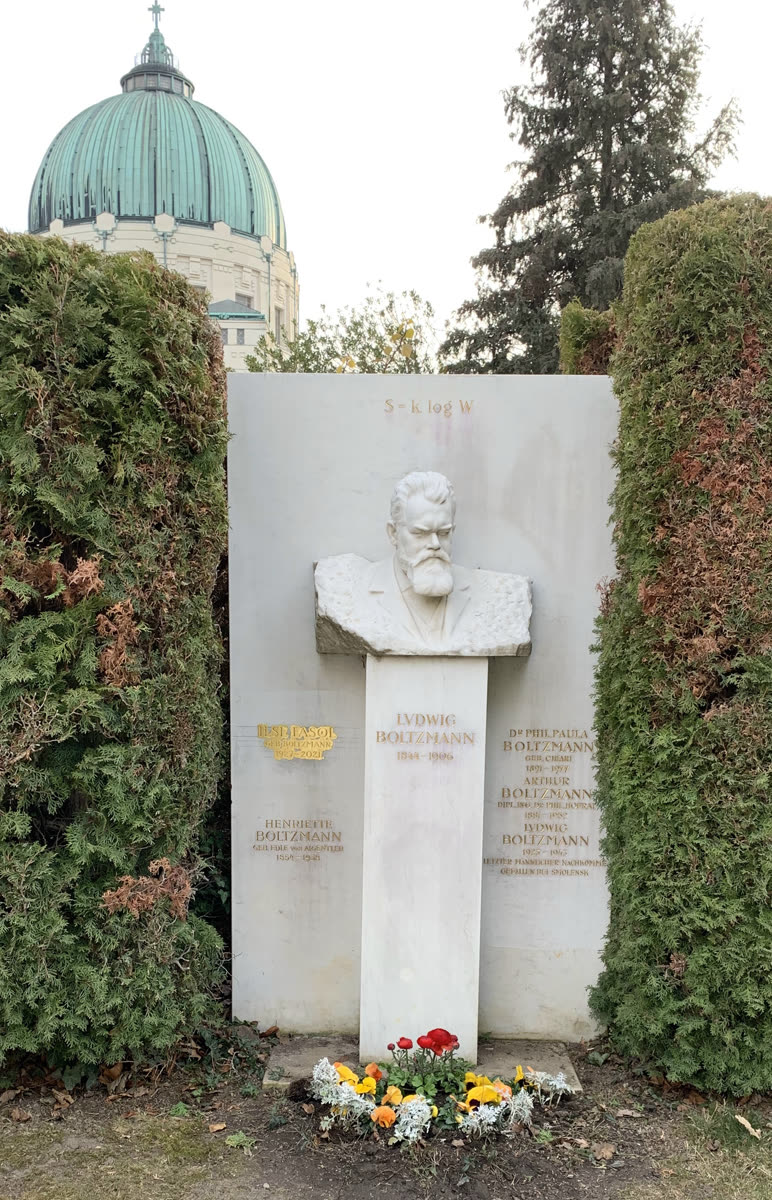
\includegraphics[width=\linewidth]{images/book4/boltzmann-grave.jpg}\par
{\footnotesize 玻尔兹曼的墓碑。}
\end{minipage}
\end{history}

\section{练习}

\begin{exercise}[$\star$]\label{exo:b3:partition-functions:1}
四个振子共享四个量子。列出各种分布，求出每种分布的权重，
并验证它们之和等于将四个不可区分的量子放入四个振子的方式数，
$\binom{7}{3}$。哪些分布是
最可几的？
\end{exercise}

\begin{exercise}[$\star$]\label{exo:b3:partition-functions:2}
两个非简并能级相距 \qty{2.5}{kJ/mol}，求它们的
布居数之比，分别在 \qty{298.15}{K} 和 \qty{1000}{K} 时。在极高
温度下，该比值的极限是多少？
\end{exercise}

\begin{exercise}[$\star$]\label{exo:b3:partition-functions:3}
% ledger: aw:Ar
计算氩原子在 \qty{298.15}{K} 时的热波长，以及
其在体积为 \qty{1}{dm^3} 时的平动配分函数。
\end{exercise}

\begin{exercise}[$\star$]\label{exo:b3:partition-functions:4}
% ledger: diat:N2.Be, diat:N2.ae, diat:HCl.Be, diat:HCl.ae
已知 $B_0 = \qty{1.990}{cm^{-1}}$（\ce{N2}）和 \qty{10.440}{cm^{-1}}（\ce{H^{35}Cl}），求二者的 $\theta_{\mathrm R}$ 以及
每种分子在
\qty{298.15}{K} 时的高温转动配分函数。
\end{exercise}

\begin{exercise}[$\star\star$]\label{exo:b3:partition-functions:5}
% ledger: diat:I2.we, diat:I2.wexe, diat:N2.we, diat:N2.wexe
\ce{I2} 和 \ce{N2} 的基频波数分别为 \qty{213.27}{cm^{-1}} 和
\qty{2329.92}{cm^{-1}}。求 $\theta_{\mathrm V}$、\qty{298.15}{K} 时的 $q^{\mathrm V}$，以及
不处于 $v = 0$ 的分子所占的比例。
\end{exercise}

\begin{exercise}[$\star\star$]\label{exo:b3:partition-functions:6}
% ledger: diat:NO.split, lev:Cl.2P1_2
求 \qty{298.15}{K} 时 \ce{NO}（两个二重
简并能级相距 \qty{119.73}{cm^{-1}}）和氯原子（基态为 ${}^2P_{3/2}$，
${}^2P_{1/2}$ 位于 \qty{882.35}{cm^{-1}}）的电子配分函数。\ce{NO} 分子中处于较高能级的比例是多少？
$q^{\mathrm E}(\ce{NO})$ 在高温下趋于何值？
\end{exercise}

\begin{exercise}[$\star\star$]\label{exo:b3:partition-functions:7}
由 $q^{\mathrm T} = V/\Lambda^3$ 推导一摩尔单原子理想气体的内能和
定容热容，并计算 $U - U(0)$ 在
\qty{298.15}{K} 时的值。
\end{exercise}

\begin{exercise}[$\star\star$]\label{exo:b3:partition-functions:8}
% ledger: aw:Ar, s0:Ar_g
用萨克尔–特特罗德方程计算氩在
\qty{298.15}{K} 时的标准摩尔熵，并与表列值
\qty{154.846}{J.K^{-1}.mol^{-1}} 比较。若压强除以 10，它会变化多少？
\end{exercise}

\begin{exercise}[$\star\star$]\label{exo:b3:partition-functions:9}
% ledger: diat:HCl.Be, diat:HCl.ae
计算 \ce{H^{35}Cl} 在 \qty{298.15}{K} 时标准摩尔熵的
转动贡献（$\theta_{\mathrm R} = \qty{15.02}{K}$）。
\end{exercise}

\begin{exercise}[$\star\star\star$]\label{exo:b3:partition-functions:10}
将 $J$ 视为连续变量，证明线型分子布居数最多的转动能级
位于 $J_{\max} = \sqrt{T/2\theta_{\mathrm R}} - \frac12$ 附近。对 \ce{HCl}
（$\theta_{\mathrm R} = \qty{15.02}{K}$）和 \ce{CO}（$\theta_{\mathrm R} = \qty{2.766}{K}$）在 \qty{300}{K} 下计算该值。
为什么红外带的两支在离中心几条谱线处最强？
\end{exercise}

\begin{exercise}[$\star\star\star$]\label{exo:b3:partition-functions:11}
% ledger: diat:H2.Be, diat:H2.ae
欧拉–麦克劳林公式给出 $\sum_{J\ge0}f(J) \approx \int_0^\infty f(J)\dd J + \frac12f(0) -
\frac1{12}f'(0)$。将其应用于 $f(J) = (2J+1)\eu^{-\theta J(J+1)/T}$，证明 $q^{\mathrm R} \approx T/\theta +
\frac13$。在哪些温度下 $T/\theta$ 的误差在 1\,\% 以内？对 \ce{H2}
（$B_0 = \qty{59.32}{cm^{-1}}$）在 \qty{298.15}{K} 下，这一近似是否可接受？
\end{exercise}

\begin{exercise}[$\star\star\star$]\label{exo:b3:partition-functions:12}
% ledger: diat:I2.we, diat:I2.wexe
证明：当 $T \ll \theta_{\mathrm V}$ 时，振动摩尔熵趋于零，而趋于
$R[1 + \ln(T/\theta_{\mathrm V})]$（当 $T \gg \theta_{\mathrm V}$ 时）。计算精确表达式及该极限
在 \qty{298.15}{K} 下对 \ce{I2}（$\theta_{\mathrm V} = \qty{306.9}{K}$）求值，并加以评论。
\end{exercise}

\section{问题：计算氮气的熵}

\begin{problem}[{周末问题——计算氮气的熵：
由光谱计算其标准熵的平动、转动、振动
和电子贡献，并与表中数据比较}]
\label{pb:b3:partition-functions:1}
% ledger: aw:N, diat:N2.Be, diat:N2.ae, diat:N2.we, diat:N2.wexe, s0:N2_g, const:h, const:kB, const:NA, const:c
氮气是空气的主要成分。其标准摩尔熵
在 \qty{298.15}{K} 下，由其摩尔质量 \qty{28.014}{g/mol}
及光谱常数计算得出：$B_e = \qty{1.998241}{cm^{-1}}$，$\alpha_e = \qty{0.017318}{cm^{-1}}$，$\omega_e =
\qty{2358.57}{cm^{-1}}$，$\omega_ex_e = \qty{14.324}{cm^{-1}}$；其电子基态项为 ${}^1\Sigma_g^+$。
标准压强 $p^\circ = \qty{1}{bar}$；$k = \qty{1.380649e-23}{J/K}$，$h = \qty{6.62607015e-34}{J.s}$。

\medskip\noindent\textbf{第一部分——平动。}
\begin{enumerate}
  \item 计算一个分子的质量。
  \item 计算其在 \qty{298.15}{K} 下的热波长。
  \item 计算每个分子可占据的体积 $kT/p^\circ$。
  \item 推出 $q^{\mathrm T}/N$，并评论其大小。
  \item 计算平动摩尔熵。
  \item 压强减半时，它将改变多少？
\end{enumerate}

\medskip\noindent\textbf{第二部分——转动。}
\begin{enumerate}[resume]
  \item 计算 $B_0$。
  \item 计算 $\theta_{\mathrm R}$。
  \item 给出对称数，并说明它所计入的内容。
  \item 计算在 \qty{298.15}{K} 下的 $q^{\mathrm R}$。
  \item 高温形式是否合理？
  \item 计算转动摩尔熵。
  \item 忽略核自旋权重，哪一个转动能级
        的布居数最大？
\end{enumerate}

\medskip\noindent\textbf{第三部分——振动与电子态。}
\begin{enumerate}[resume]
  \item 计算振动量子 $G(1) - G(0)$。
  \item 计算 $\theta_{\mathrm V}$。
  \item 计算在 \qty{298.15}{K} 下的 $q^{\mathrm V}$。
  \item 处于 $v = 1$ 的分子占多大比例？
  \item 计算振动摩尔熵。
  \item 电子贡献是多少？为何可以
        忽略激发电子态？
\end{enumerate}

\medskip\noindent\textbf{第四部分——求和与比较。}
\begin{enumerate}[resume]
  \item 将各项贡献相加。
  \item 与表中所列的 \qty{191.609}{J.K^{-1}.mol^{-1}} 比较。
  \item 表中的量热熵值依据哪些测量？
  \item 表格为何可以不计核自旋？
  \item 给出结果：氮气在 \qty{298.15}{K} 下的标准摩尔熵，
        由其光谱常数计算得出。
\end{enumerate}
\end{problem}
